\documentclass[../../LearnCpp.tex]{subfiles}

\begin{document}

\asubsection{3}{Order of construction of derived classes}

\begin{lstlisting}[language=C++]
class Base
{
public:
    int m_id {};

    Base(int id=0)
        : m_id { id }
    {
    }

    int getId() const { return m_id; }
};

class Derived: public Base
{
public:
    double m_cost {};

    Derived(double cost=0.0)
        : m_cost { cost }
    {
    }

    double getCost() const { return m_cost; }
};
\end{lstlisting}

这个例子中 \acode{Derived} 由 \acode{Base} 中派生出来。

\begin{figure}[h]
    \centering
    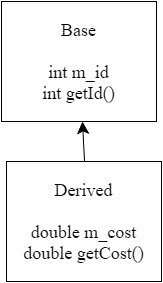
\includegraphics[width=3cm]{\subfix{../images/DerivedBase}}
    \label{fig:DerivedBase}
    \caption{DerivedBase}
\end{figure}

因为 \acode{Derived} 从 \acode{Base} 中继承了函数与变量,
也许可能会认为 \acode{Base} 的成员被拷贝到了 \acode{Derived}。
然而这并不正确。相反的是 \acode{Derived} 被视为两部分的类:
一部分是 \acode{Derived},另一部分是 \acode{Base}。

\begin{figure}[h]
    \centering
    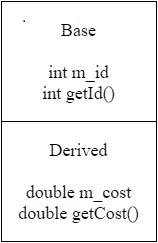
\includegraphics[width=3cm]{\subfix{../images/DerivedBaseCombined}}
    \label{fig:DerivedBaseCombined}
    \caption{DerivedBaseCombined}
\end{figure}

当 C++ 构造派生对象时:首先最开始的类(即继承树最顶层)被构造,
接着每个子类按照顺序依次构造,直到最底层的类(继承树的最底层)被构造。

\begin{lstlisting}[language=C++]
#include <iostream>

class Base
{
public:
    int m_id {};

    Base(int id=0)
        : m_id { id }
    {
        std::cout << "Base\n";
    }

    int getId() const { return m_id; }
};

class Derived: public Base
{
public:
    double m_cost {};

    Derived(double cost=0.0)
        : m_cost { cost }
    {
        std::cout << "Derived\n";
    }

    double getCost() const { return m_cost; }
};

int main()
{
    std::cout << "Instantiating Base\n";
    Base base;

    std::cout << "Instantiating Derived\n";
    Derived derived;

    return 0;
}
\end{lstlisting}

打印:

\begin{lstlisting}
Instantiating Base
Base
Instantiating Derived
Base
Derived
\end{lstlisting}

\subsubsection*{继承链的构造顺序}

\begin{lstlisting}[language=C++]
#include <iostream>

class A
{
public:
    A()
    {
        std::cout << "A\n";
    }
};

class B: public A
{
public:
    B()
    {
        std::cout << "B\n";
    }
};

class C: public B
{
public:
    C()
    {
        std::cout << "C\n";
    }
};

class D: public C
{
public:
    D()
    {
        std::cout << "D\n";
    }
};

int main()
{
    std::cout << "Constructing A: \n";
    A a;

    std::cout << "Constructing B: \n";
    B b;

    std::cout << "Constructing C: \n";
    C c;

    std::cout << "Constructing D: \n";
    D d;
}
\end{lstlisting}

记住 C++ 总是最先构建”最初“或者”最基础“的类。
接着通过继承树的顺序来构造每个派生类。打印:

\begin{lstlisting}
Constructing A:
A
Constructing B:
A
B
Constructing C:
A
B
C
Constructing D:
A
B
C
D
\end{lstlisting}

\end{document}
